\documentclass{scrartcl}
\usepackage{fullpage}
\usepackage{pdfpages}
\usepackage{graphicx}

\setlength{\parindent}{0.0in}
\setlength{\parskip}{0.1in}

\addtolength{\topmargin}{-1cm}
\addtolength{\textheight}{2cm}

\title{Human Centred Design}
\subtitle{CALMist - The Elimination of Stress in our Day to Day Living}
\author{Christopher Bowles, Jack Bracewell, Craig Ellis,\\David Harrison, Karl Kely, Milan Misak, Daniel Randall}
\date{}

\begin{document}
\maketitle
\tableofcontents
\clearpage

\section{Abstract}
Stress is a common factor in people's lives. It affects their ability to work and play, and can have serious health
implications, especially if left unchecked. Interviewing a number of employees of certain firms, it is clear that
people want a solution, but are not always aware when it is that they are most stressed. We propose a couple of
wearable devices that measure stress throughout the day, with a gamified companion website to provide feedback,
stress-reducing tips and encouragement.

\section{Problem Statement}
Personal well-being and happiness is a priority for everyone.
Stress is one of the leading causes of illness and depression in the country.
In order to provide a solution to provide a high quality service at a minimal cost,
we need to produce an unobtrusive user friendly product to improve quality of life.

\section{The Impact of Stress}
Stress is the adverse reaction people have to excessive pressures or other types of demand placed on them.
It is one of the leading causes for health issues in the modern world, and has implications for
employees, employers and the health system.

For employees, a study showed that 75\% of illnesses that required the employee to take time off work were
the direct result of stress. Coupled with the fact that people sufferring from excessive stress spend around 50\%
more on medical expenses in America, we can see that this puts an enormous strain on health services, especially
if we consider countries like the UK, where the figure is probably similar but the health system is publicly funded.
Surprisingly, another study shows that only about 40\% of people in the UK describe their job as stressful. However,
given the number of complaints we heard during the interview process, we question this figure.

For employers, the obvious problem is that they are losing work (as employees take stress-related sick leave) and thus
potentially money. To put this in perspective, in the 2009/10 business year, an estimated 9.8 million working days
were lost in the UK due to work-related stress. This puts stress-related sick leave above strokes, heart attacks and
cancer as a cause of extended workplace absence. It isn't much of a stretch of the imagination to reckon that this
probably results in something of a viscious cycle. People are stressed at work so they need sick leave. Less work gets
done because so many people are taking stress-related sick leave. When they get back, looming deadlines mean more work
in a shorter amount of time, which leads to more stress, and thus more health issues and sick leave, and so on and so forth.

\section{Interviews Process}
When we identified our problem we needed to be able to create a realistic persona
in order to develop for. To this end we needed to find out about real people
who have experienced stress. To facilitate this we decided that we should
develop questionaires and go out and talk to people about stress and get them to 
fill this out. A lot of people talked to us but didn't want to fill out the 
questionaire.

In the appendix I have included a few of the responses we got. Below is the 
questionaire in question:

\fbox{
\setlength{\fboxsep}{0pt}
\setlength{\fboxrule}{1pt}
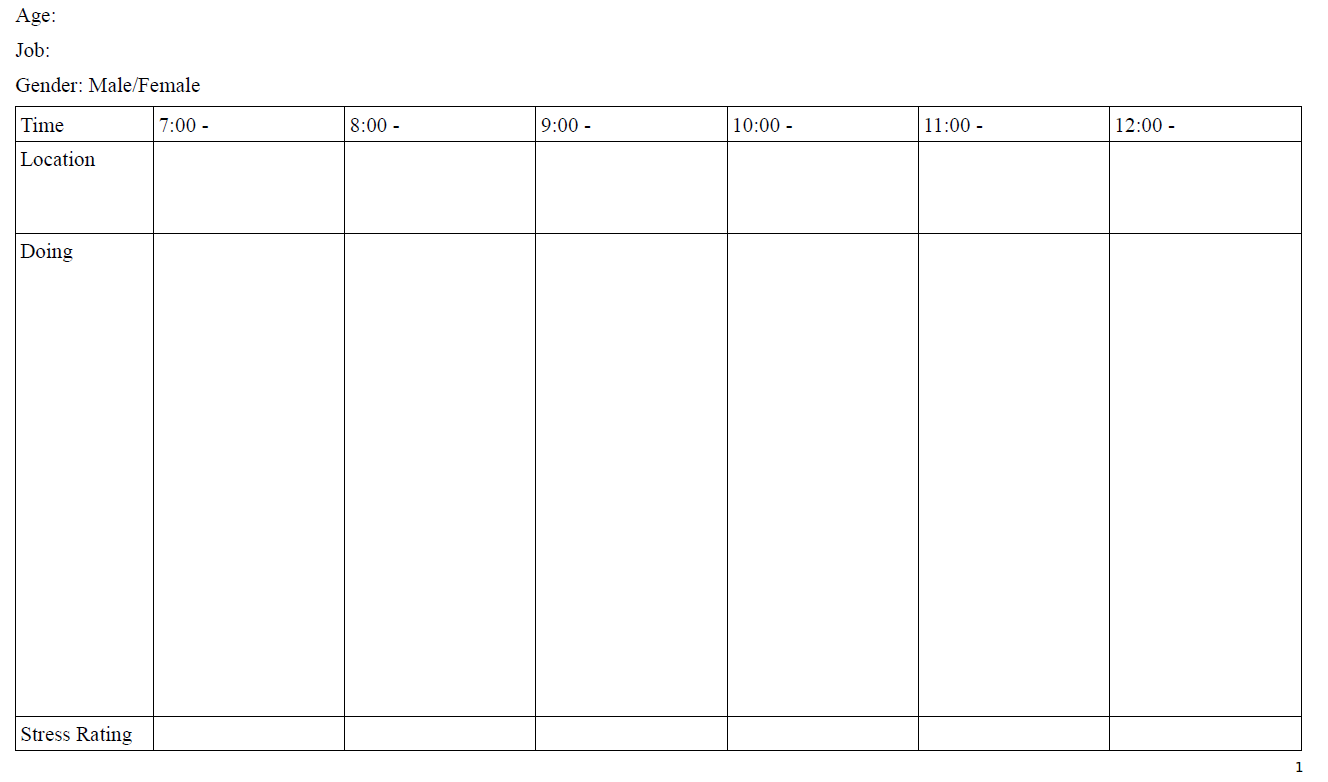
\includegraphics[scale=0.3]{PDFResponses/Templatepg1x.png}
}

\fbox{
\setlength{\fboxsep}{0pt}
\setlength{\fboxrule}{1pt}
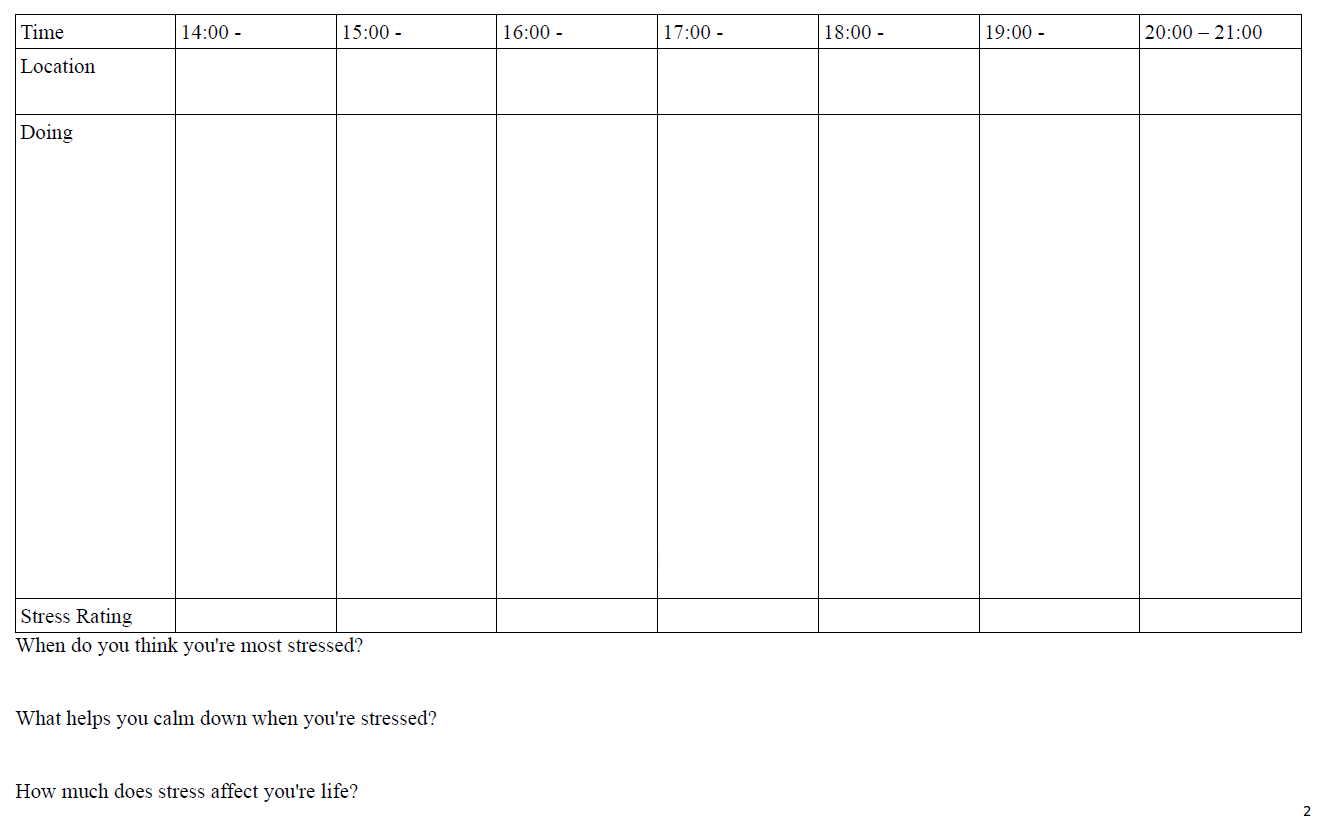
\includegraphics[scale=0.3]{PDFResponses/Templatepg2x.png}
}

\section{Interview Results}
The interviews suprised us a lot. From it we realised that stress
affected many more people than what you would expect. For example 
one of the people we interviewed revealed to us that he actually
had a psychologist to help him deal with his stress. This was
suprising considering the job the person had, a clerk at Ryman.
This isn't a job which would normally be considered high stress
however this person needed to get a psychologist to help him cope.

Another person we interviewed worked at Kodak, his responses were 
equally surprising. At the start of his day he spent about two hours
stress managedment activities such as yoga and breathing exercises.
He also had attended seminars about coping with stress.

We interviewed a library assisstant as well at one point. She 
herself didn't suffer to badly from stress throughout the day
but she did tell us that the most stressful time of day for her was
actually travelling to and from work. This was interesting as
none of us had considered that travelling was a trigger for stress.
We brought this up with other people we interviewed and they told
us that travelling was very stressful for them as well. The
interesting thing though is that they themselves hadn't realised
that travelling was stressing them out until they were asked by
us.

The main things we took from this was that stress affected much
more people than most people realise and that even if you aren't
in a high stress job, your job can be very stressful. Also 
quite a lot of people don't even realisewhat it is that stresses
them unless its pointed out to them. This information was used
in both the design of our persona, Lydia, and in the development 
of the solution.

\section{Our Persona - Lydia}

\section{Development of our Idea}
After interviewing people and developing the persona we were going to focus on, we decided we were ready to try and come up with
a solution. In total, we came up with 2 ideas that we eventually rejected, and combined what we felt were the best elements
of the two into our final solution.

\subsection{Idea 1 - Self Help Website}
Our first idea was what can only be described as a self-help website. Users would log on to read tips, and we would attempt to
design everything around the idea of calm (so using light blue and/or green colours, as they are commonly deemed relaxing,
and gentle wording). The website would also have a user forum, so people can talk to others about their problems and advise
other people (something that in itself can be quite calming).

However, although this sounds like a decent solution on paper, we saw a number of problems with it.
For a start, it does not take the user's emotional needs into account. Stress is a very personal thing, and people do not
tend to want to talk about it. Indeed, we found we were very often turned down when trying to interview people during the
interview stage. It's true that the internet allows for a certain anonymity, and sometimes it's actually easier to talk
about personal things with complete strangers, but there's still always going to be that sense of taboo about talking about
such things, as well as the feeling of vulnerability the users will likely feel by opening up. As such, we don't think users
are that likely to actually open up, which means the forum would not be used to it's full potential. Indeed it may actually
discourage the potential user from using the service at all, despite the forum being optional. Stress is a very delicate
topic, and this idea just isn't sensitive enough.

Furthermore, except for the
forum element, it's not particularly interactive. It's essentially just an online book. Yes things could be added to it, and we
could implement features such as "tip of the day", but it's still passively reading about stress avoidance. This may well be
enough for some people, but we doubt it would be for most. It in no way encourages people through the more stressful times or
motivates them to improve themselves. What would be needed is some way of making it more active and engaging. The obvious
solution would be gamification. However, we're not really sure how you can gamify this. A point for every tip you read?
That would just turn it into a study game, and in no way measure actual progress or give any indication of how stressed the user
is/is not. The system needs to actively measure the user's progress to provide the needed level of interaction. This lead
us on to our second idea.

\subsection{Idea 2 - Stress Alerts}
Our second idea was some form of wearable device, such as a bracelet. It would be constantly measuring your stress levels.
Research shows that skin conductance varies with stress, along with breathing pattern. As such, this device would measure
skin conductance. The idea is that it would have a mini alarm, and alert you when your stress levels become ''too high``
(a subjective property, so of course some calibration would probably be required).

This certainly does solve the problem of lack of quantification present in the previous idea, so we didn't want to drop
the idea entirely. However, there is one very big and obvious problem. This, too, isn't sensitive enough to the user's
delicate state, but rather than being too passive like the first idea, it's far too agressive.

Consider someone who is currently in a period of high stress. Perhaps they've just been fired, or perhaps a subordinate has
done something incorrectly and caused them a lot more work. If you're fired, you probably need a short period of ''grief``
to get back on your feet, and yes, if someone has messed up, getting stressed about it is unproductive. But now imagine what
affect adding a device saying "you are stressed" would have.

When people are stressed, they don't want to be told they are stressed. They may want any manner of thing, but awareness
is seldom one of them. Hence, having an alarm that goes off when they are stressed is likely to just make them even more
stressed. It would make a bad situation worse. Hence, this idea in its present form was quickly rejected. The method of
measurement and quantification did, however, go on to form the backbone of our final idea.

\subsection{Final Idea}

As we learnt from research into our second idea, stress can be quantified by measuring skin conductance and breathing pattern.
The user needs to be given feedback based upon actual real-world measurements, but it's counter-productive to do this in
real-time. Hence, for our final idea, we proposed maintaining the idea of constant measurement for analysis,
but completely abandoning the idea of real-time feedback, instead opting for end-of-the-day at-the-user's-leisure feedback.

What we mean by this is that we still have a device that measures stress through skin conductance.
These measurements will be somehow uploaded
to a computer (details of implementation are in following sections). The computer would then let the user view a simplified version
of the readings to see how their stress levels varied throughout the day. This would also, obviously, let them see when
they were most stressed, and trivially but worth a mention, low stress.

It's true that people don't always know what exact circumstances cause them to be stress, but with so much emphasis on the
negative, people seem to even more often not know what causes them to be calm. With the ability to review stress levels throughout
the day, the user can identify periods of high stress, link it to a situation and try to avoid similar circumstances. However,
just as importantly, they can also identify periods of calm, link those to situations, and try to actively seek out
similar situations. Both of these actions should have positive health implications.

In terms of interactivity, this system makes it relatively easy to converse with and encourage the user. Now that we have
a definitive figure for stress, it is relatively easy to gamify. What we proposed was that we take some aggregate of the
recorded stress levels throughout the day and present this as a score. The user can then compare their day's score with their
previous scores.


\section{Measuring Stress}
\subsection{Existing Devices}
\subsection{Our Proposed Devices}

\section{Giving Feedback - Personalised, Gamified Website}
\subsection{Website Concept}
\subsection{Gamification}

\section{Value Proposition}

\section{Stakeholder Summary}

\section{Appendix - Questionaires}
Here are a few of the sample responses we got from our questionaires.
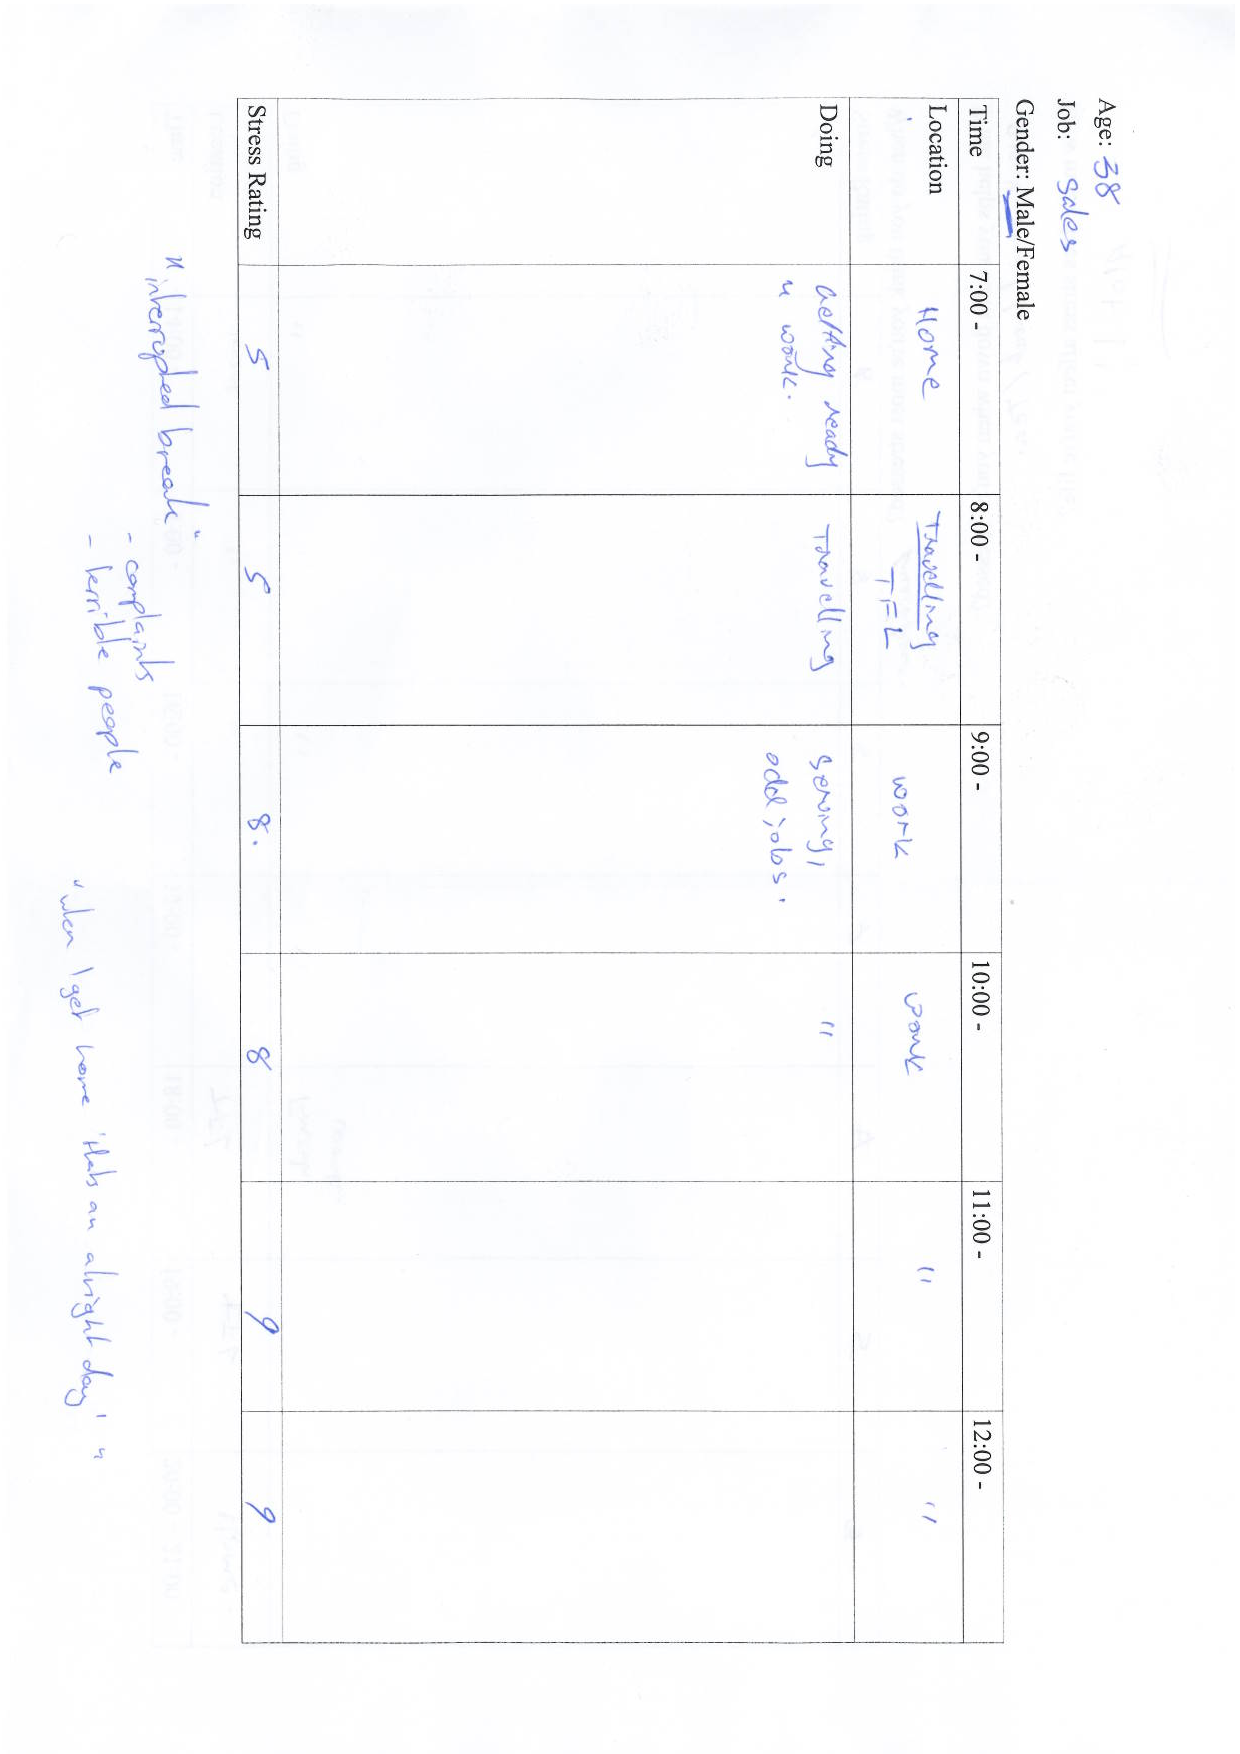
\includepdf{PDFResponses/Ryman1}
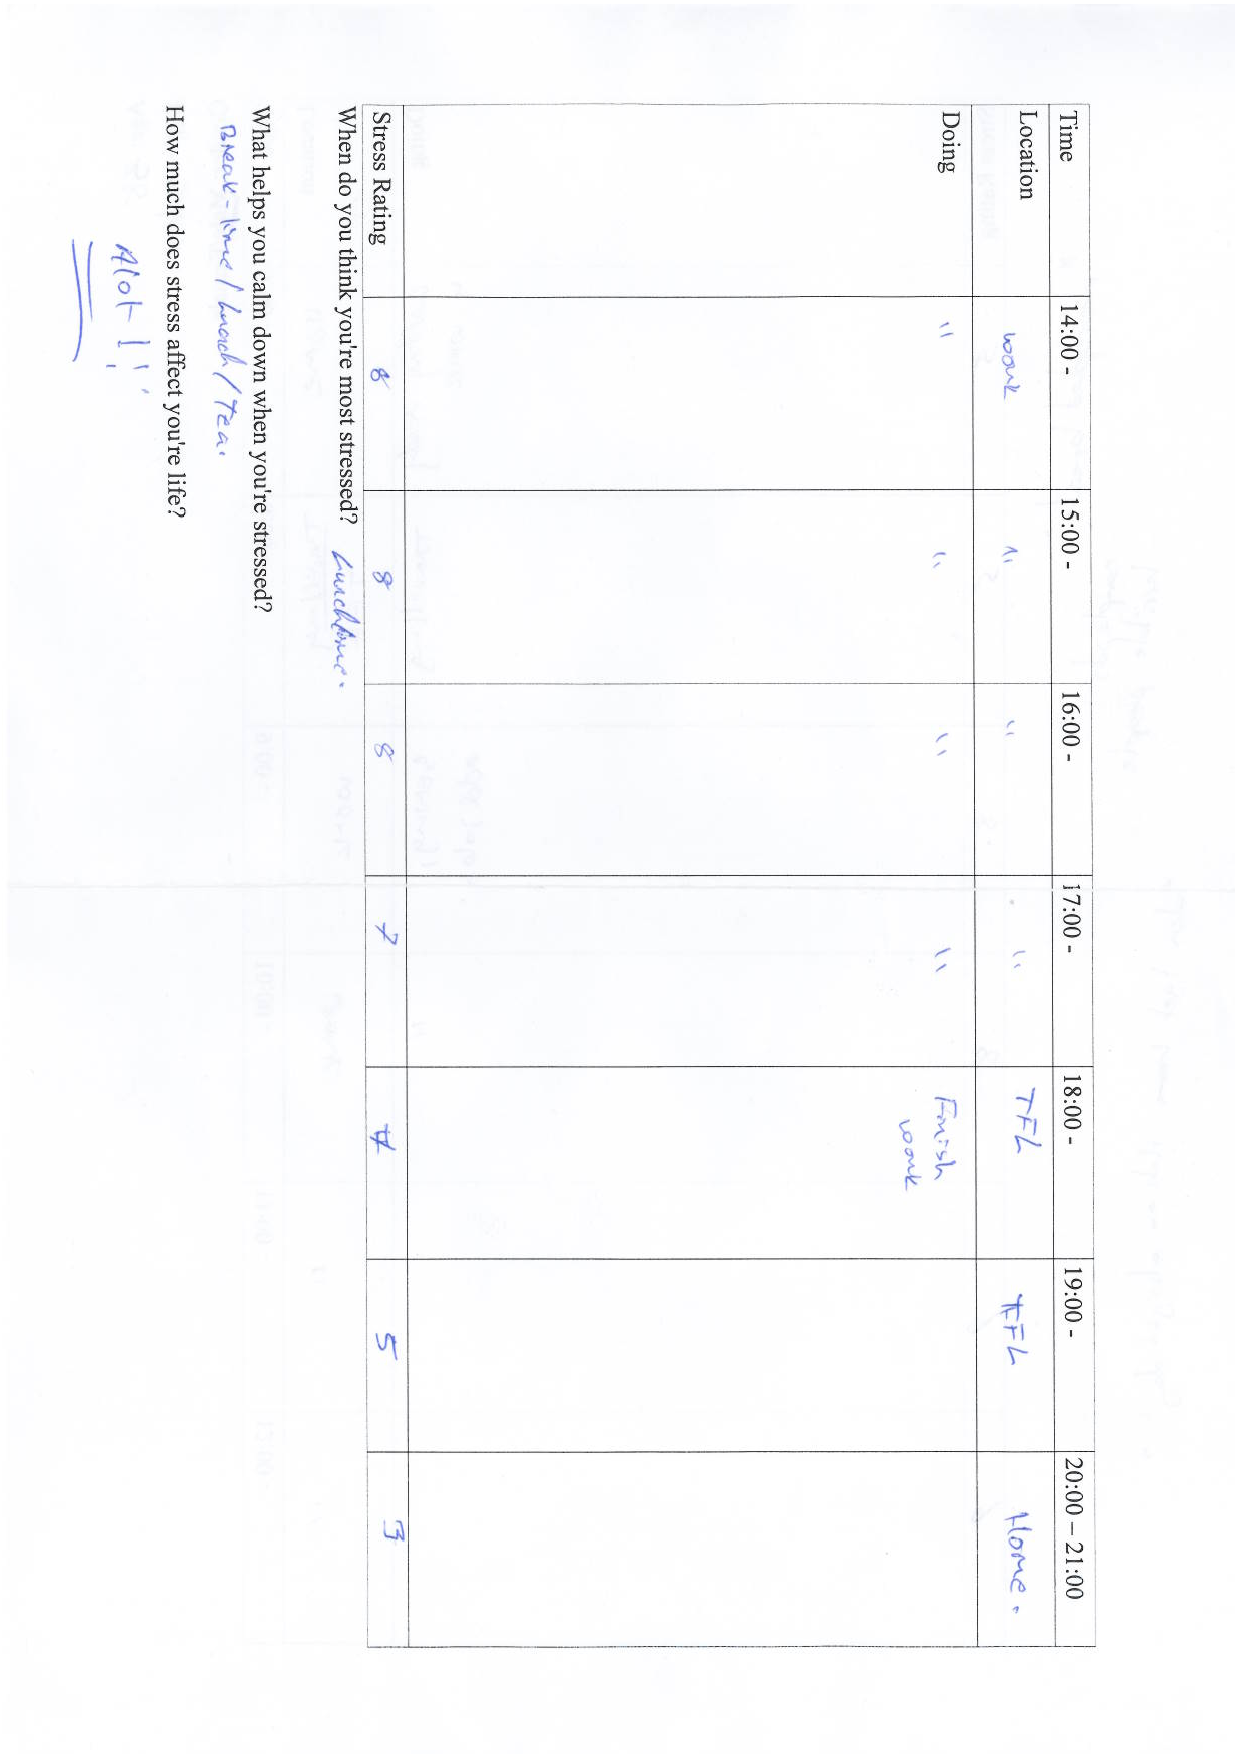
\includepdf{PDFResponses/Ryman2}
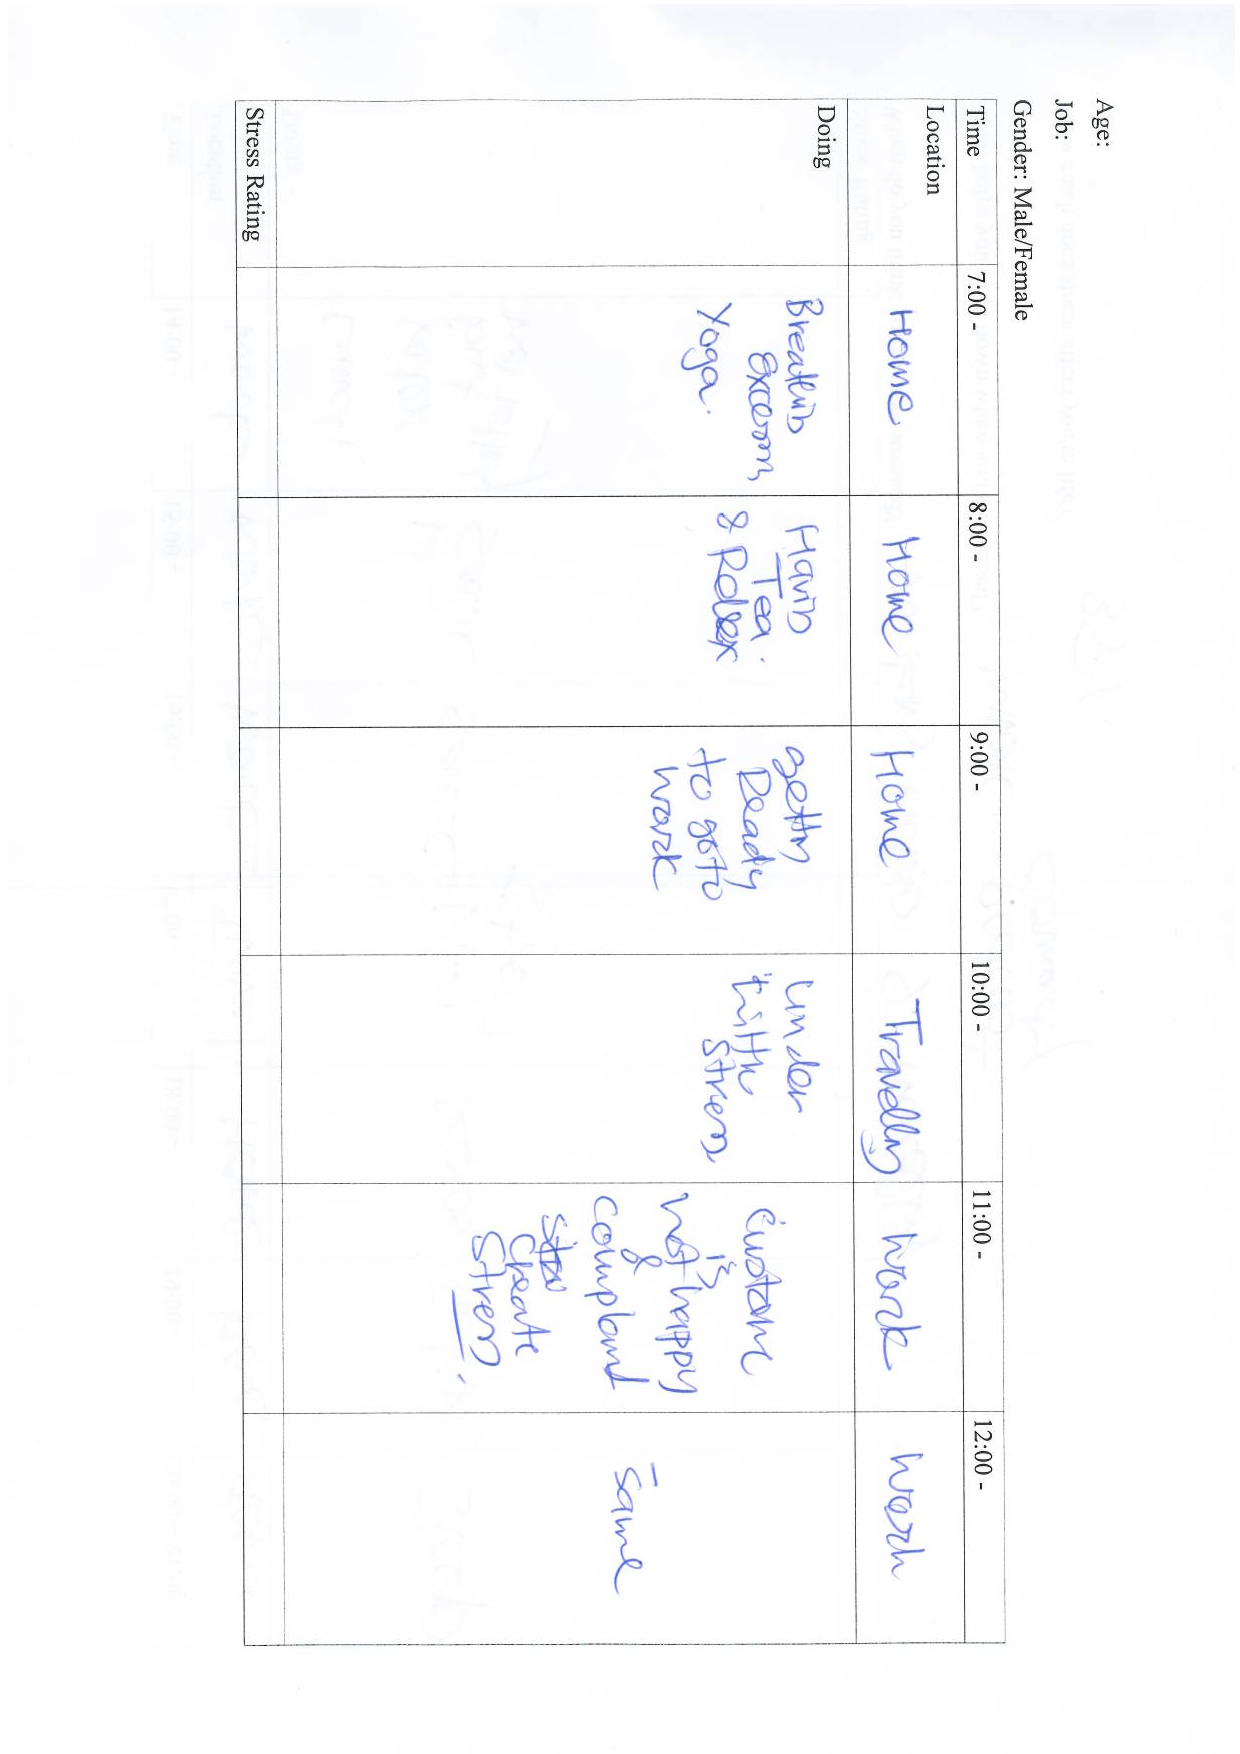
\includepdf{PDFResponses/Kodak1}
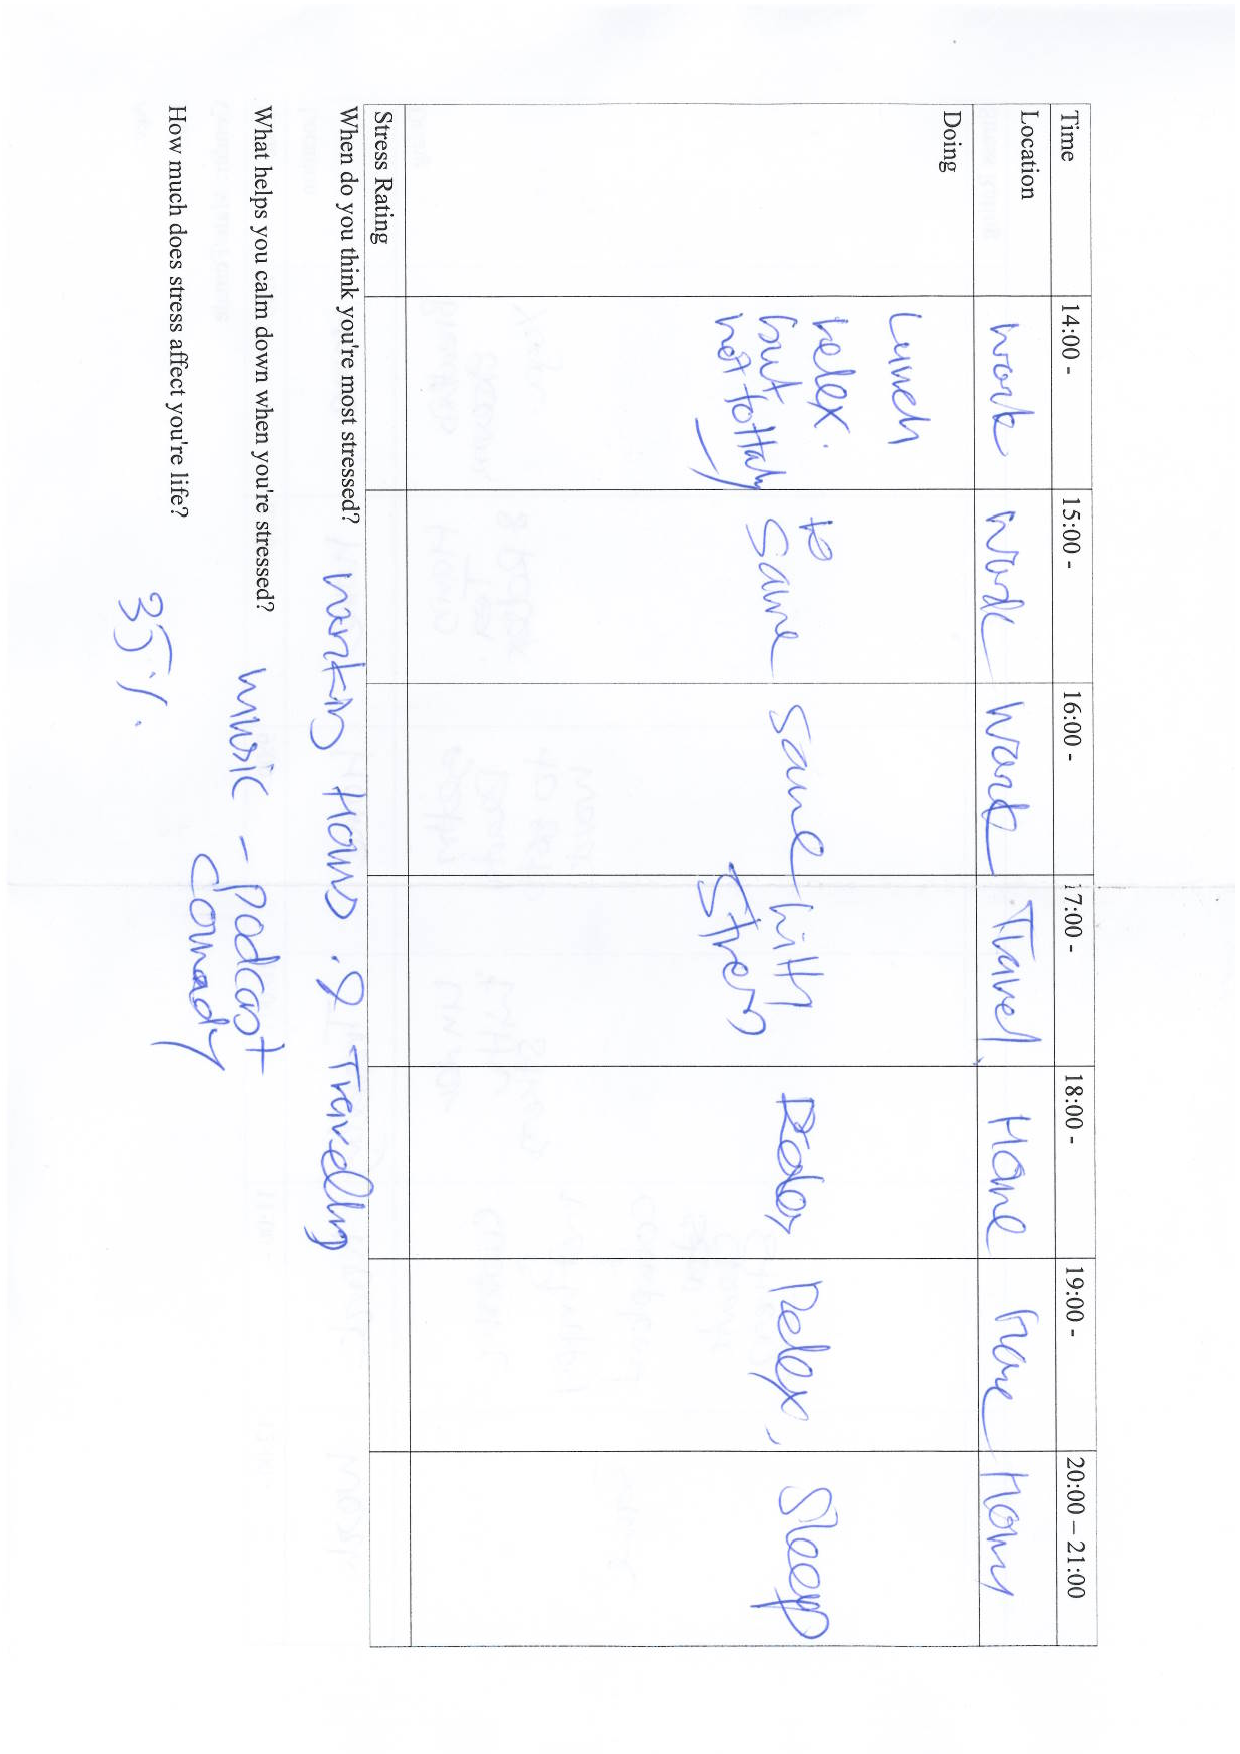
\includepdf{PDFResponses/Kodak2}
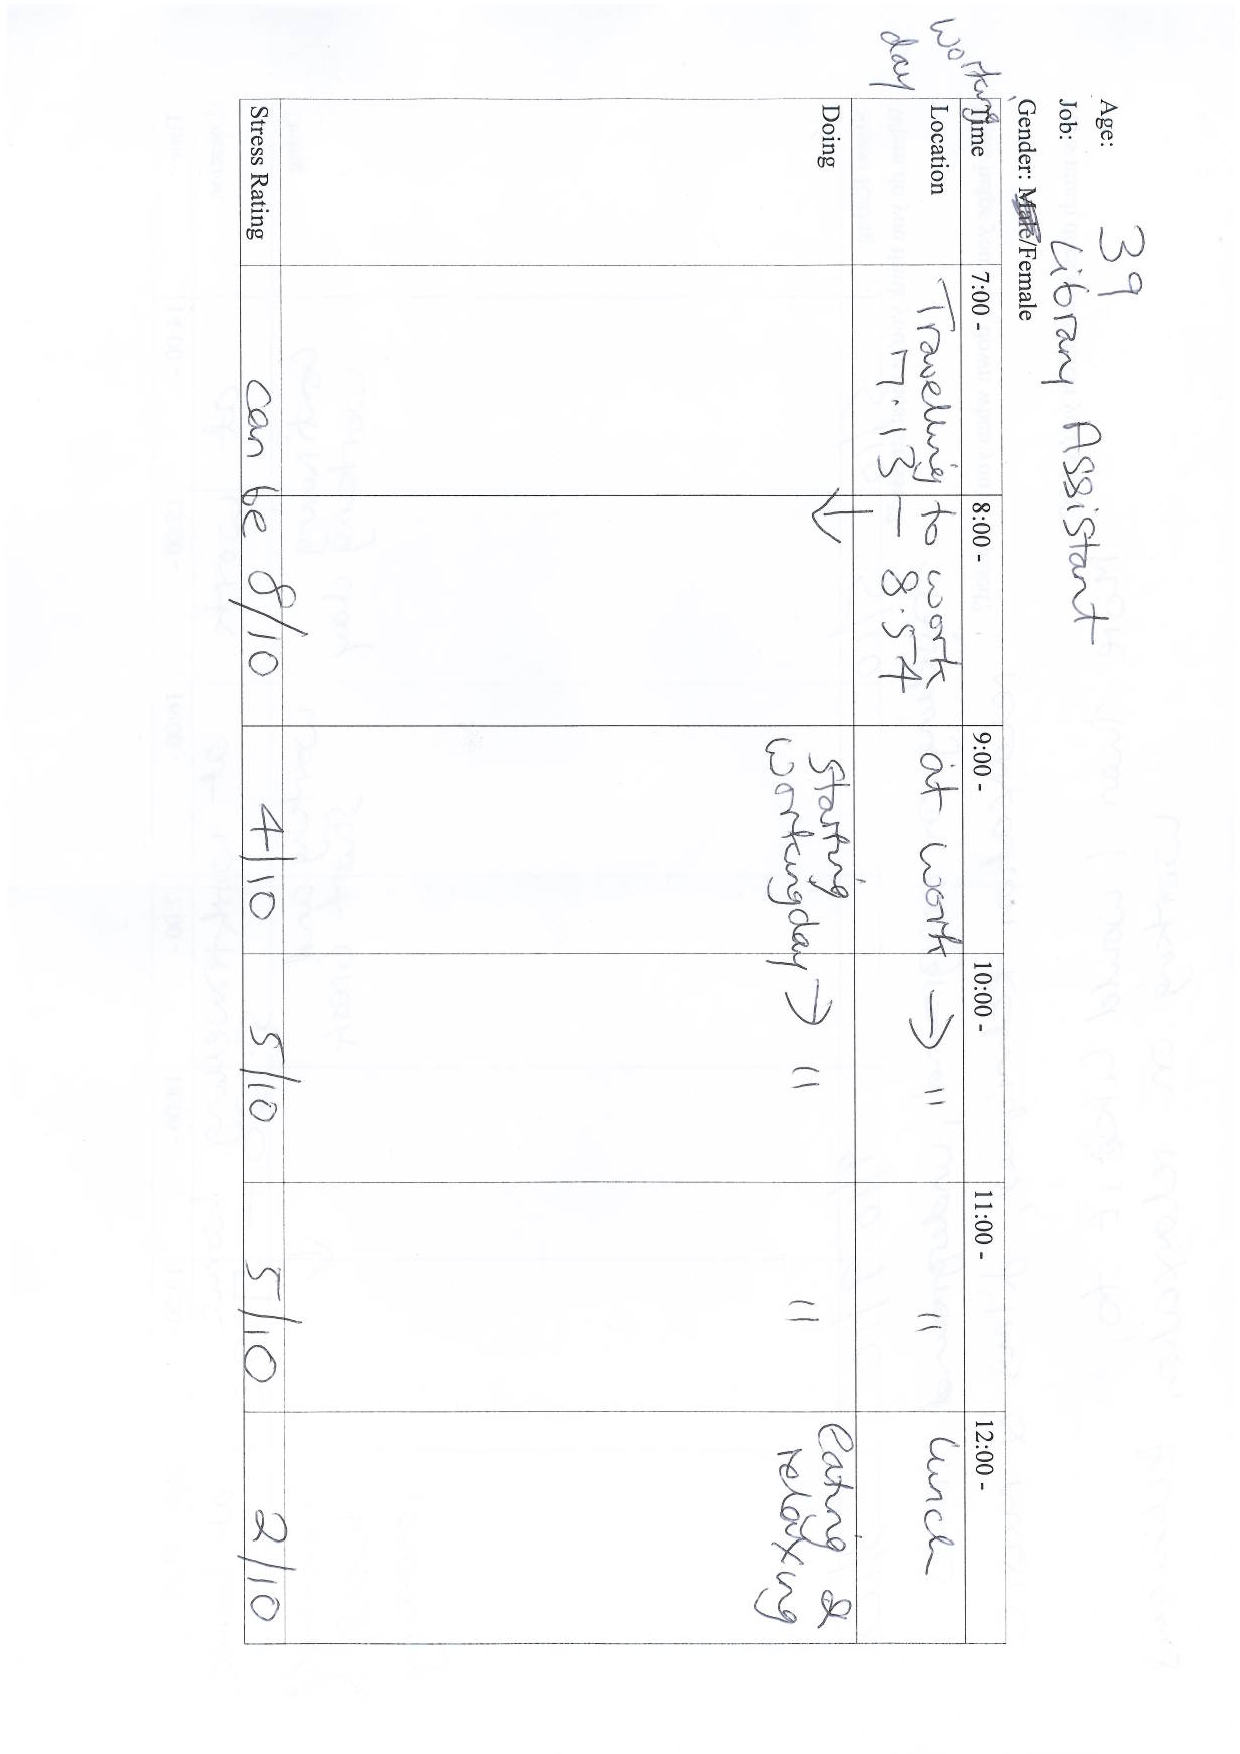
\includepdf{PDFResponses/LibraryAssistant1}
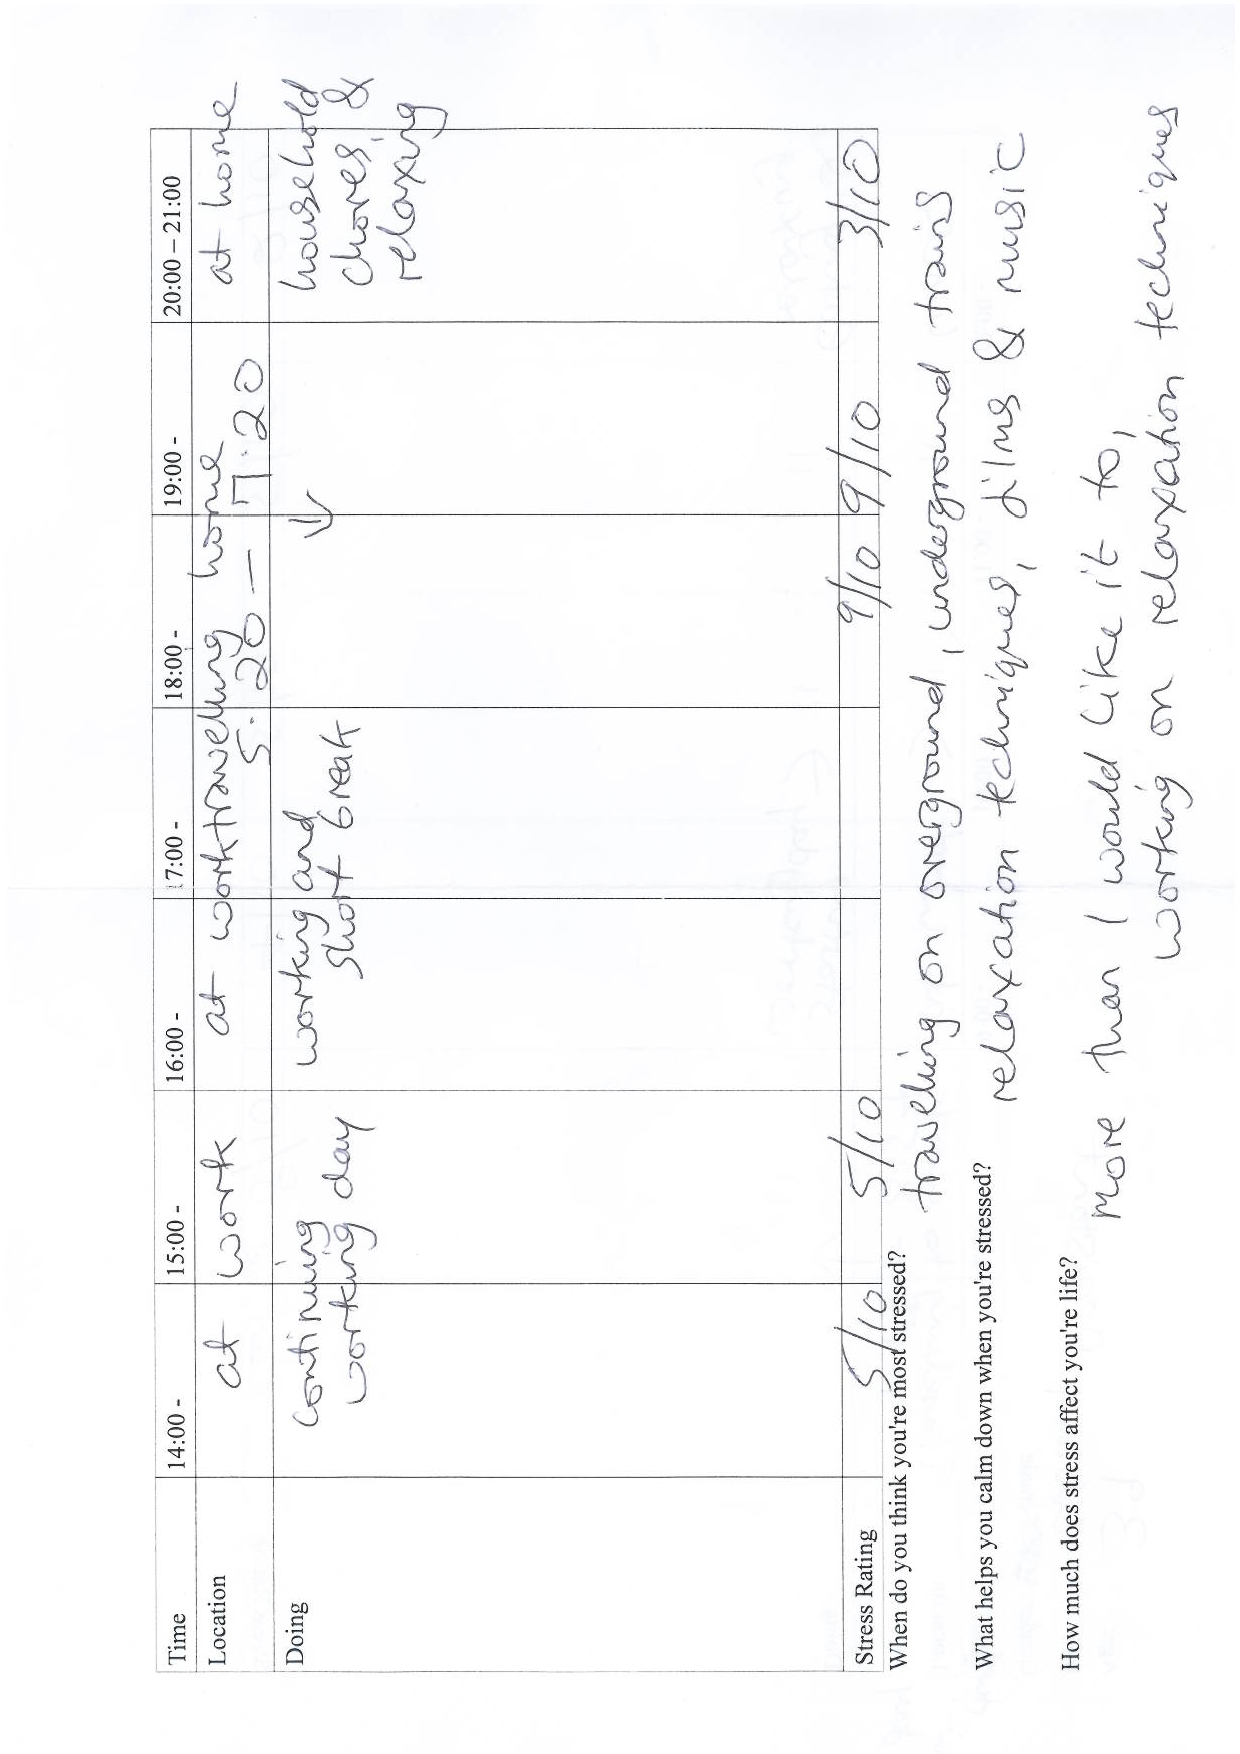
\includepdf[angle=180]{PDFResponses/LibraryAssistant2}
\end{document}
